\documentclass[12pt,aspectratio=169]{beamer}

\usetheme[
    sectionpage=progressbar,
    subsectionpage=progressbar,
    progressbar=frametitle
]{metropolis}

\definecolor{blue-grey-900}{HTML}{263238}
\definecolor{deep-orange-500}{HTML}{FF5722}
\setbeamercolor{normal text}{fg=blue-grey-900, bg=white}
\setbeamercolor{alerted text}{fg=deep-orange-500}

\usepackage{graphicx}
\usepackage{hyphenat}
\usepackage[normalem]{ulem}

\usepackage{polyglossia}
\setdefaultlanguage[variant=british]{english}
\usepackage[english=british]{csquotes}

\usepackage{fontspec}
\setmainfont{Lucida Sans OT}
\setsansfont[Scale=MatchLowercase]{Lucida Sans OT}
\setmonofont[Scale=MatchLowercase]{Lucida Console DK}
\defaultfontfeatures{Ligatures=TeX}

\title{MLOps --- from Prototyping to Production}
\author{Gianluca Campanella}
\date{6\textsuperscript{th} June 2019}

\begin{document}

\maketitle

\begin{frame}{Hello!}
    \begin{center}
        \LARGE%
        My name is \textbf{Gianluca}
        {\fontspec{Gentium}\textcolor{gray}{[dʒanˈluːka]}}
    \end{center}
\end{frame}

\begin{frame}{What I do nowadays}
    \LARGE%
    \only<1>{%
        \begin{center}
            I'm a Data Scientist at \\[\bigskipamount]
            
\includegraphics[height=2.5em]{figures/microsoft} \\[\medskipamount]
            in \textbf{AzureCAT}
        \end{center}}
    \only<2>{%
        \begin{center}
            I also run my own company \\[\bigskipamount]
            \raisebox{-0.5\height}{
\includegraphics[height=2.5em]{figures/estimand}}
            \raisebox{-0.5\height}{\huge Estimand} \\[\medskipamount]
            that provides \\
            \textbf{Data Science consulting and training}
        \end{center}}
\end{frame}

\begin{frame}{Today we're talking about\ldots}
    \begin{center}
        {\Huge%
         MLOps}
        \vfill\pause
        ($\approx$ a whole bunch of mistakes I made in the last few years)
    \end{center}
\end{frame}

\begin{frame}{Things I've helped build recently}
    \begin{itemize}
        \setlength{\itemsep}{\bigskipamount}%
        \item High\hyp{}frequency trading system for sports betting
        \item Context\hyp{}aware, personalised search engine
        \item Content recommender for a mobile app
        \item Automated forecasting tool for an e\hyp{}commerce business
    \end{itemize}
\end{frame}

\begin{frame}{Two types of Data Science}
    \begin{columns}
        \begin{column}{0.5\textwidth}
            \begin{center}
                \large\bf%
                Analysis\hyp{}focused
            \end{center}
            \begin{itemize}
                \item Maths and Statistics
                \item Business Intelligence
                \item[$\to$] Assist human decision\hyp{}making
            \end{itemize}
        \end{column}
        \begin{column}{0.5\textwidth}
            \begin{center}
                \large\bf%
                Building\hyp{}focused
            \end{center}
            \begin{itemize}
                \item Machine Learning
                \item Software Engineering
                \item[$\to$] Develop and deploy data\hyp{}driven products
            \end{itemize}
        \end{column}
    \end{columns}
\end{frame}

\begin{frame}{Don't try to run before you can walk}
    \begin{center}
        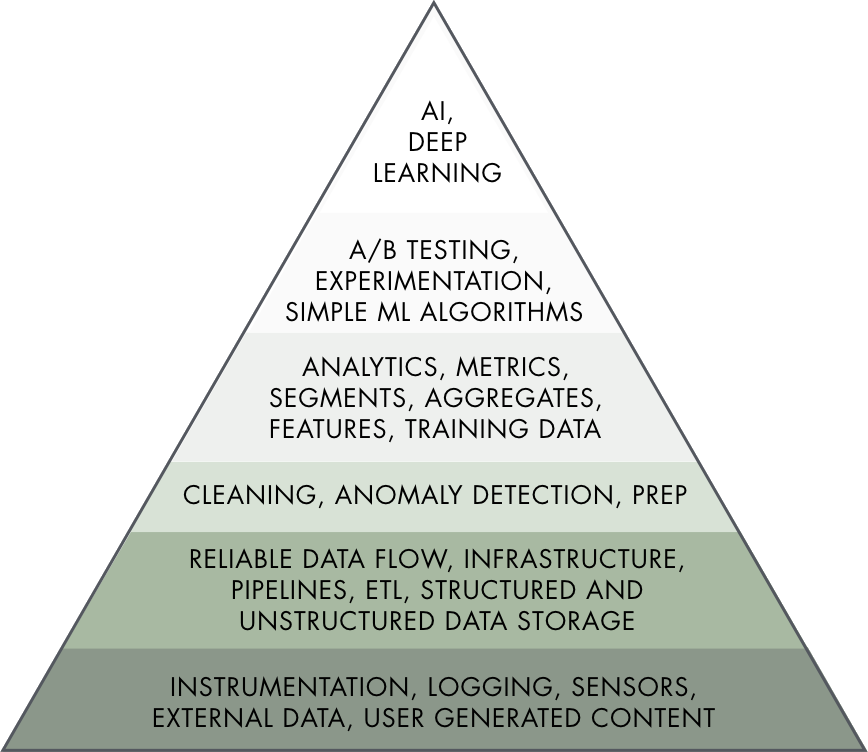
\includegraphics[height=0.8\textheight]{figures/ai_hierarchy} \\
        {\scriptsize%
         From M.\ Rogati}
    \end{center}
\end{frame}

\begin{frame}
    \only<1>{%
        \begin{center}
            \LARGE%
            What is MLOps?
        \end{center}}
    \only<2>{%
        \begin{center}
            \LARGE%
            What is DevOps?
        \end{center}}
\end{frame}

\begin{frame}{DevOps}
    \only<1>{%
        \begin{block}{What?}
            Automation practices between software developers and IT
        \end{block}
        \vfill
        \begin{block}{Why?}
            To build, test and release software faster and more reliably
        \end{block}}
    \only<2>{%
        \begin{quote}
            At its essence, DevOps is a culture, a movement, a philosophy.

            \begin{flushright}
                    --- Atlassian
            \end{flushright}
        \end{quote}}
\end{frame}

\begin{frame}{MLOps}
    \begin{block}{What?}
        Automation practices between \alert{data scientists},
        \alert{data engineers}, software developers and IT
    \end{block}
    \vfill
    \begin{block}{Why?}
        To build, test, release and \alert{monitor} software that
        \alert{embeds ML} faster and more reliably
    \end{block}
\end{frame}

\begin{frame}
    \begin{center}
        \LARGE%
        Why does this matter?
    \end{center}
\end{frame}

\begin{frame}{Why does this matter?}
    \only<1>{%
        \Large%
        \begin{center}
            High\hyp{}risk, high\hyp{}reward innovation culture
            \vfill
            $\downarrow$
            \vfill
            Iterate quickly $\ \longleftrightarrow\ $ Fail fast
        \end{center}}
    \only<2>{%
        \begin{center}
            {\Large%
             If it's not used in production\ldots}
            \vfill
            {\LARGE\bf%
             It never happened!}
        \end{center}}
    \only<3>{%
        \begin{center}
            {\Large%
             If \emph{it is} used in production\ldots}
            \vfill
            {\LARGE\bf%
             It better work!}
        \end{center}}
    \only<4>{%
        \begin{block}{As a Data Scientist, MLOps\ldots}
            \begin{itemize}
                \item Is hard but does pay off
                \item Gives you peace of mind
                \item Allows you to focus on more interesting tasks
            \end{itemize}
        \end{block}}
    \only<5>{%
        \begin{block}{As a Software Engineer, MLOps\ldots}
            \begin{itemize}
                \item Is something you're probably already doing
                \item Increases the dependability of ML systems
                \item Brings you closer to the Data Science team
            \end{itemize}
        \end{block}}
\end{frame}

\begin{frame}{Where are we in the DS workflow?}
    \only<1>{%
        \begin{center}
            \large%
            Research question
            \vfill
            $\downarrow$
            \vfill
            Obtain $\ \longleftrightarrow\ $ Explore $\ \longleftrightarrow\ $ Model
            \vfill
            $\downarrow$
            \vfill
            Operationalise
        \end{center}}
    \only<2>{%
        \begin{center}
            \large%
            Research question
            \vfill
            $\downarrow$
            \vfill
            Obtain $\ \longleftrightarrow\ $ Explore $\ \longleftrightarrow\ $ Model
            \vfill
            $\downarrow$
            \vfill
            \alert{Operationalise}
        \end{center}}
    \only<3>{%
        \begin{center}
            \large%
            Research question
            \vfill
            $\downarrow$
            \vfill
            \alert{Obtain} $\ \longleftrightarrow\ $ Explore $\ \longleftrightarrow\ $ \alert{Model}
            \vfill
            $\downarrow$
            \vfill
            \alert{Operationalise}
        \end{center}}
    \only<4>{%
        \begin{center}
            \large%
            Data sources
            \vfill
            $\downarrow$
            \vfill
            ETL $\ \longleftrightarrow\ $ Model development $\ \longleftrightarrow\ $ Training
            \vfill
            $\downarrow$
            \vfill
            Deployment
        \end{center}}
    \only<5>{%
        \begin{center}
            \large%
            Data sources
            \vfill
            $\downarrow$
            \vfill
            \alert{ETL} $\ \longleftrightarrow\ $ Model development $\ \longleftrightarrow\ $ \alert{Training}
            \vfill
            $\downarrow$
            \vfill
            \alert{Deployment}
        \end{center}}
\end{frame}

\begin{frame}
    \begin{center}
        \large%
        Data sources
        \vfill
        $\downarrow$
        \vfill
        \alert{ETL} $\ \longleftrightarrow\ $ Model development $\ \longleftrightarrow\ $ Training
        \vfill
        $\downarrow$
        \vfill
        Deployment
    \end{center}
\end{frame}

\begin{frame}{ETL}
    \only<1>{%
        \begin{block}{What?}
            \begin{itemize}
                \item \textbf{E}xtract, \textbf{T}ransform, \textbf{L}oad
                \item Data Science alchemy
                \item Heavily informed by domain knowledge and EDA
            \end{itemize}
        \end{block}}
    \only<2>{%
        \begin{block}{Things to keep in mind}
            \begin{itemize}
                \item Distributional assumptions
                \item Transformations
                \item External data sources
            \end{itemize}
        \end{block}}
\end{frame}

\begin{frame}
    \begin{center}
        \large%
        Data sources
        \vfill
        $\downarrow$
        \vfill
        ETL $\ \longleftrightarrow\ $ \alert{Model development} $\ \longleftrightarrow\ $ Training
        \vfill
        $\downarrow$
        \vfill
        Deployment
    \end{center}
\end{frame}

\begin{frame}{Model development}
    \only<1>{%
        \begin{block}{How?}
            \begin{itemize}
                \item Hyperparameter tuning
                \item Automated ML
            \end{itemize}
        \end{block}}
    \only<2>{%
        \begin{block}{Things to keep in mind}
            \begin{itemize}
                \item Choice of programming language
                \item Versioning
                \item Performance tracking
            \end{itemize}
        \end{block}}
    \only<3>{%
        \centering%
        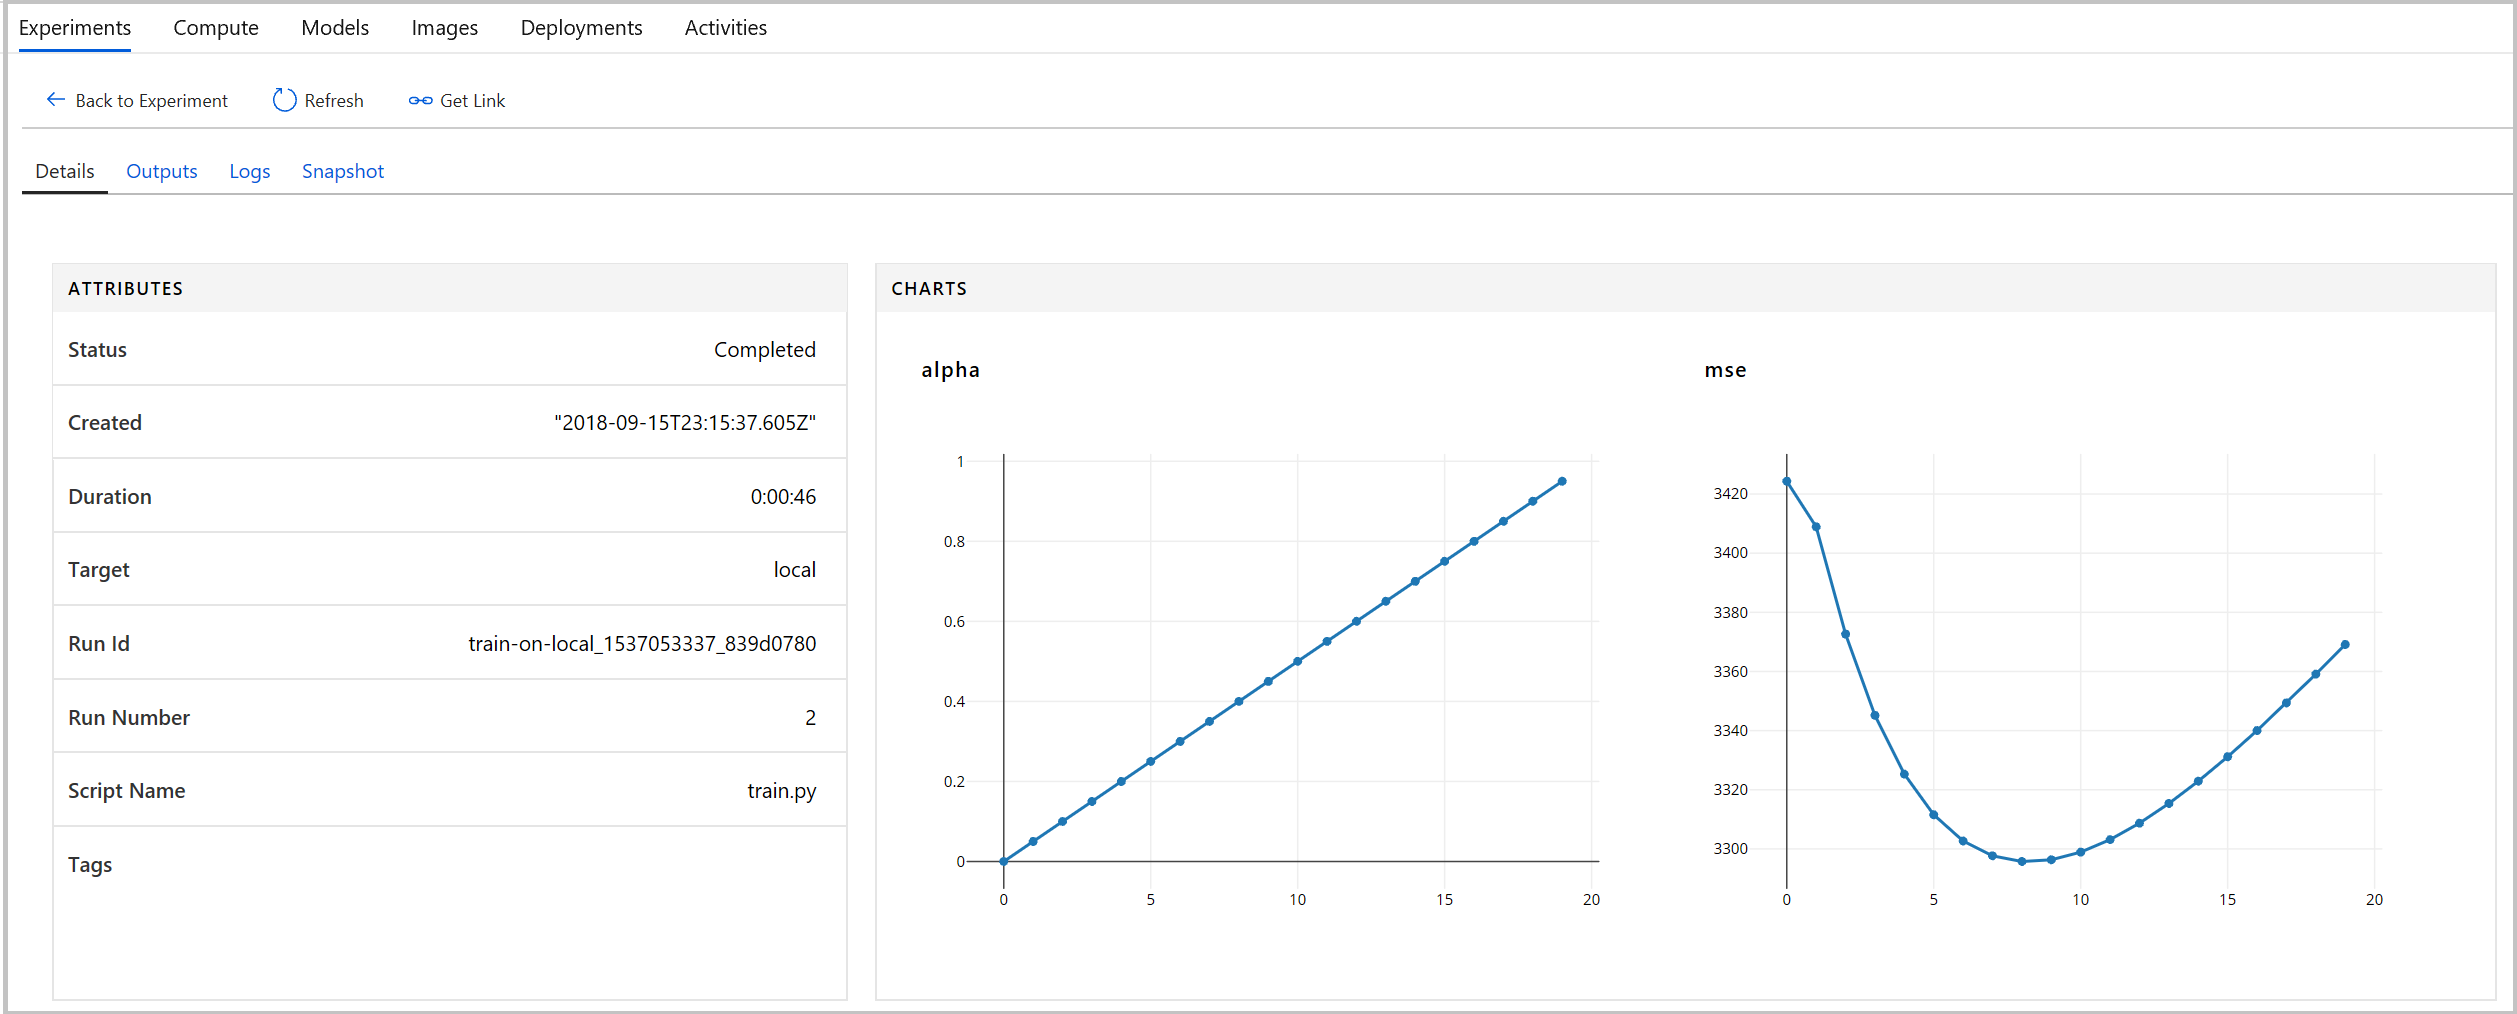
\includegraphics[width=\textwidth]{figures/aml_run_details}}
\end{frame}

\begin{frame}{\textit{Interlude}}
    \only<1>{%
        \begin{block}{Online vs offline metrics}
            \begin{itemize}
                \item Business metrics $\to$ online metrics
                \item Offline metrics $\approx$ online metrics
                \item Experiment early and often
            \end{itemize}
        \end{block}}
    \only<2>{%
        \begin{block}{Feedback loops}
            \begin{itemize}
                \item Models become self\hyp{}fulfilling prophecies
                \item Biased data collection
                \item Explore\hyp{}exploit trade\hyp{}off
            \end{itemize}
        \end{block}}
\end{frame}

\begin{frame}
    \begin{center}
        \large%
        Data sources
        \vfill
        $\downarrow$
        \vfill
        ETL $\ \longleftrightarrow\ $ Model development $\ \longleftrightarrow\ $ \alert{Training}
        \vfill
        $\downarrow$
        \vfill
        \alert{Deployment}
    \end{center}
\end{frame}

\begin{frame}{Training vs scoring}
    \begin{block}{Training}
        \begin{itemize}
            \item Historical data $\to$ model
            \item Scheduled offline (batch) jobs
        \end{itemize}
    \end{block}
    \vfill\pause
    \begin{block}{Scoring}
        \begin{itemize}
            \item Model + new data $\to$ predictions
            \item Online or offline (batch)
        \end{itemize}
    \end{block}
\end{frame}

\begin{frame}{Deployment}
    \only<1>{%
        \begin{block}{How?}
            \begin{itemize}
                \item Offline (batch) scoring
                \item Queues
                \item RPC (e.g.\ REST endpoint)
                \item In\hyp{}process
            \end{itemize}
        \end{block}}
    \only<2>{%
        \begin{block}{Things to keep in mind}
            \begin{itemize}
                \item Throughput and latency requirements
                \item Impedance mismatch between training and scoring%
                      \textsuperscript{$\star$}
                \item Access control and security
                \item Other moving parts (e.g.\ databases)
            \end{itemize}
        \end{block}
        {\tiny%
         \textsuperscript{$\star$} I'm looking at you, Apache Spark}}
\end{frame}

\begin{frame}{Online deployment}
    \only<1>{%
        \begin{block}{How?}
            \begin{itemize}
                \item Docker
                \item Kubernetes
                \item CI/CD pipeline
            \end{itemize}
        \end{block}}
    \only<2>{%
        \begin{block}{Things to keep in mind}
            \begin{itemize}
                \item Splitting traffic
                \item A/B testing
                \item Incremental roll\hyp{}out
            \end{itemize}
        \end{block}}
\end{frame}

\begin{frame}
    \only<1>{%
        \begin{center}
            \large%
            Data sources
            \vfill
            $\downarrow$
            \vfill
            \alert{ETL} $\ \longleftrightarrow\ $ \alert{Model development} $\ \longleftrightarrow\ $ \alert{Training}
            \vfill
            $\downarrow$
            \vfill
            \alert{Deployment}
        \end{center}}
    \only<2>{%
        \begin{center}
            \LARGE%
            So\ldots~we're done?
        \end{center}}
    \only<3>{%
        \begin{center}
            {\LARGE%
             Not quite!}
            \vfill
            We still need to \alert{automate} ETL and training
        \end{center}}
\end{frame}

\begin{frame}{Retraining}
    \begin{block}{Things to keep in mind}
        \begin{itemize}
            \item Data drift
            \item Performance tracking
            \item Golden set $\to$ gated deployment
        \end{itemize}
    \end{block}
\end{frame}

\begin{frame}{Monitoring}
    \only<1>{%
        \begin{itemize}
            \item Logging
                  \begin{itemize}
                      \item Data drift
                      \item Statistical performance
                      \item Serving performance
                  \end{itemize}
            \item Anomaly detection and alerting
            \item Fallback mechanisms
        \end{itemize}}
    \only<2>{%
        \centering%
        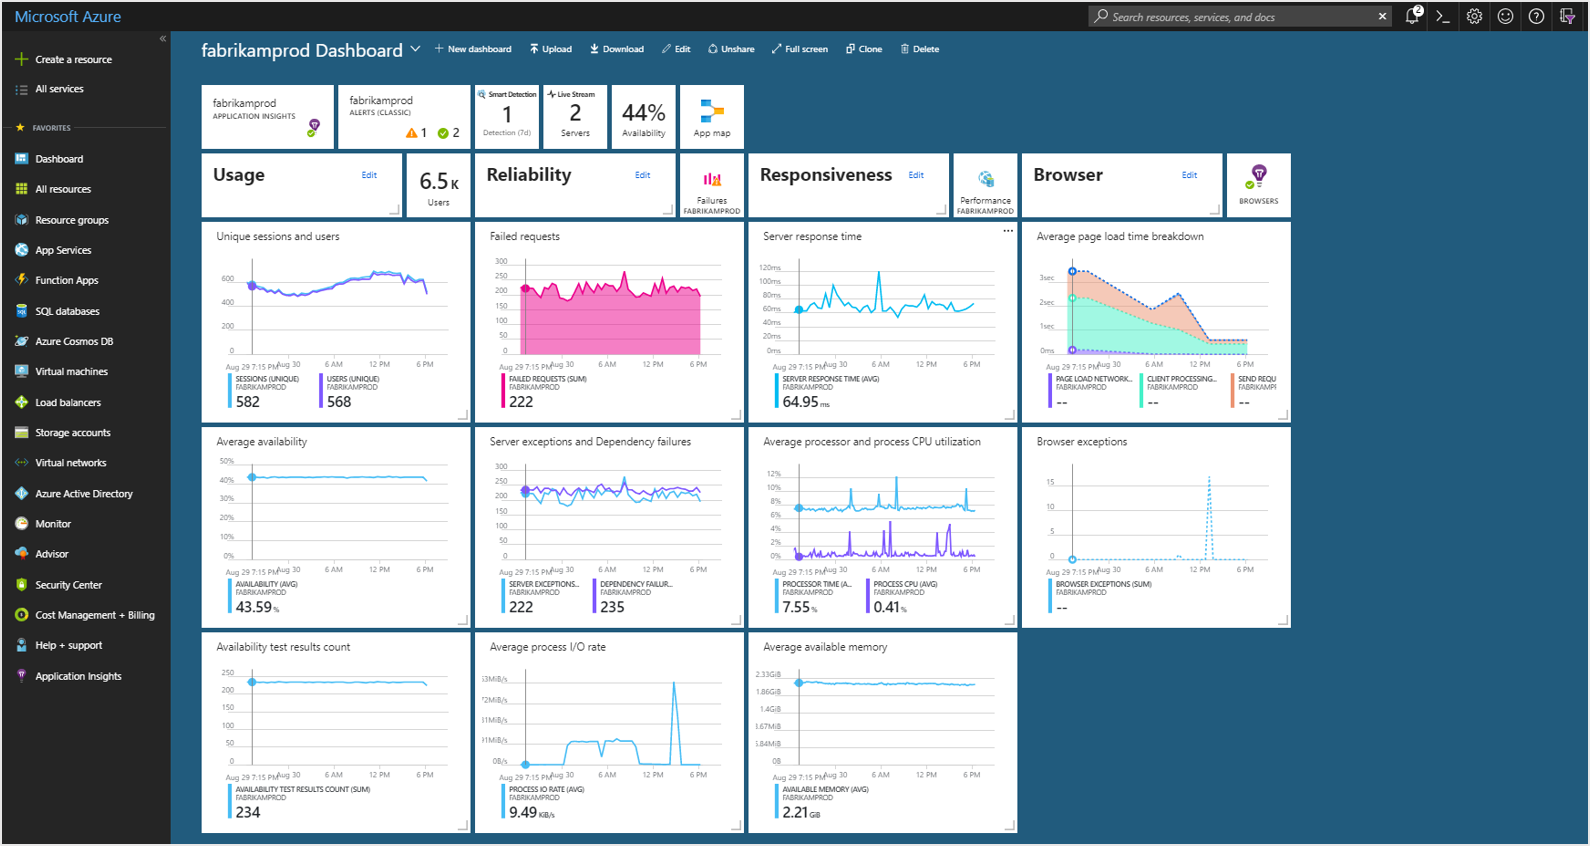
\includegraphics[width=\textwidth]{figures/app_insights_dashboard}}
\end{frame}

\begin{frame}
    \only<1>{%
        \begin{center}
            \LARGE%
            Now we're really done!
        \end{center}}
    \only<2>{%
        \begin{center}
            \LARGE%
            But then\ldots
        \end{center}}
\end{frame}

\begin{frame}{Do it again!}
    \begin{itemize}
        \item Versioning
        \item Roll\hyp{}back mechanisms
        \item Experimentation
    \end{itemize}
\end{frame}

\begin{frame}{Recap}
    \only<1>{%
        \begin{center}
            \large%
            Data sources
            \vfill
            $\downarrow$
            \vfill
            ETL $\ \longleftrightarrow\ $ Model development $\ \longleftrightarrow\ $ (Re)training
            \vfill
            $\updownarrow$
            \vfill
            Experimentation $\ \longleftrightarrow\ $ Deployment $\ \longleftrightarrow\ $ Monitoring
        \end{center}}
    \only<2>{%
        \begin{block}{As a Data Scientist\ldots}
            \begin{itemize}
                \item Familiarise yourself with the tools
                \item Try moving some of your workloads away from your laptop
                \item Understand where Engineering is coming from
            \end{itemize}
        \end{block}}
    \only<3>{%
        \begin{block}{As a Software Engineer\ldots}
            \begin{itemize}
                \item Ramp up on containers and orchestration
                \item Check out the different cloud offerings
                \item Help your fellow Data Scientists
            \end{itemize}
        \end{block}}
\end{frame}

\begin{frame}
    \begin{center}
        {\LARGE%
         Thank you!}
        \vfill
        If you want to keep in touch\ldots \\[\medskipamount]
        
\includegraphics[height=1ex]{figures/mail}~gianluca@campanella.org
        \hspace{1em}
        
\includegraphics[height=1ex]{figures/github}~gcampanella
        \hspace{1em}
        
\includegraphics[height=1ex]{figures/linkedin}~gcampanella
    \end{center}
\end{frame}

\end{document}
